\documentclass[11pt]{article}
\usepackage{graphicx, amsmath, amssymb,enumerate,listings}
\usepackage[height=9in,width=7in]{geometry}
\usepackage{url}
\usepackage{tikz}
\usetikzlibrary{trees}
\usepackage{tikz}
\usepackage{graphicx, amsmath, amssymb,enumerate,listings}
\usepackage[height=9in,width=7in]{geometry}
\usetikzlibrary{automata,positioning}

\begin{document} 
\noindent
CSC420Assignment 2 \\
By: Ou Ye 999768327\\

\noindent
\textbf{1.a} 
\begin{lstlisting}[
  mathescape,
  columns=fullflexible,
  basicstyle=\fontfamily{ttdefault}\selectfont,
]
% read image and grayscale
im = imread('./building.jpg');

hsize = 3;
sigma = 2;
result = myHarrisCornerMetric(im, hsize, sigma);
imagesc(result);

function Result = myHarrisCornerMetric(inputImage, hsize, sigma) 

    % Grayscale image
    img = rgb2gray(inputImage);

    % Compute Gradients I_x, I_y
    [Gx, Gy] = imgradientxy(img);

    % Get I_x^2, I_y^2, I_x*I_y
    Ix2 = Gx.^2;
    Iy2 = Gy.^2;
    Ixy = Gx.*Gy;

    % Gassusian Filter
    g = fspecial('gaussian', [hsize hsize], sigma);
    
    % Compute M = [Ix2g, Ixyg; Ixyg, Iy2g];
    Ix2g = conv2(Ix2, g, 'same');
    Iy2g = conv2(Iy2, g, 'same');
    Ixyg = conv2(Ixy, g, 'same');

    [h,w] = size(img);
    Result = zeros(size(img));

    for x = 1:h
        for y = 1:w
            % M for each pixel
            M = [Ix2g(x,y) Ixyg(x,y);
                Ixyg(x,y) Iy2g(x,y)];

            % Corneress with Harmonic Mean
            R = det(M) / trace(M);
            Result(x,y) = R;
        end
    end
    
    % Filter 
    Threshold = 0;
    Result(Result <= Threshold) = 0;
end

\end{lstlisting}

\begin{figure}[h]
  \caption{Result}
    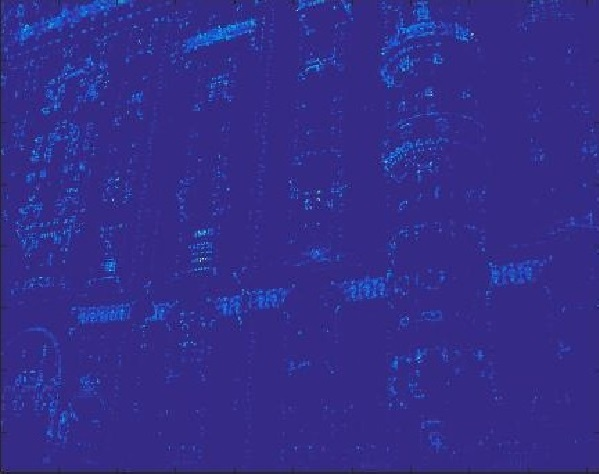
\includegraphics[width=1\textwidth]{1a}
\end{figure}

\newpage
\noindent
\textbf{1.b} \\
\begin{lstlisting}[
  mathescape,
  columns=fullflexible,
  basicstyle=\fontfamily{ttdefault}\selectfont,
]
% read image and grayscale
img = imread('./building.jpg');

hsize = 3;
sigma = 1;
Result = myHarrisCornerMetric(im, hsize, sigma);

threshold = 0.1;
radius = 1;
result = myNonMaximumSuppression(R, threshold, radius);
[X, Y] = find(result == 1);
figure;
imshow(img);
hold on;
plot(Y ,X ,'R.');

function result = myNonMaximumSuppression(R, threshold, radius) 
    domain = strel('disk', radius, 0);
    domain = domain.getnhood();
    Rmax = max(max(R));
    threshold = Rmax * threshold;
    filteredR = ordfilt2(R, sum(domain(:)), domain);
    result = filteredR > threshold;
end

\end{lstlisting}

\begin{figure}[h]
  \caption{Result with $ radius = 1, 3 ,5$}
    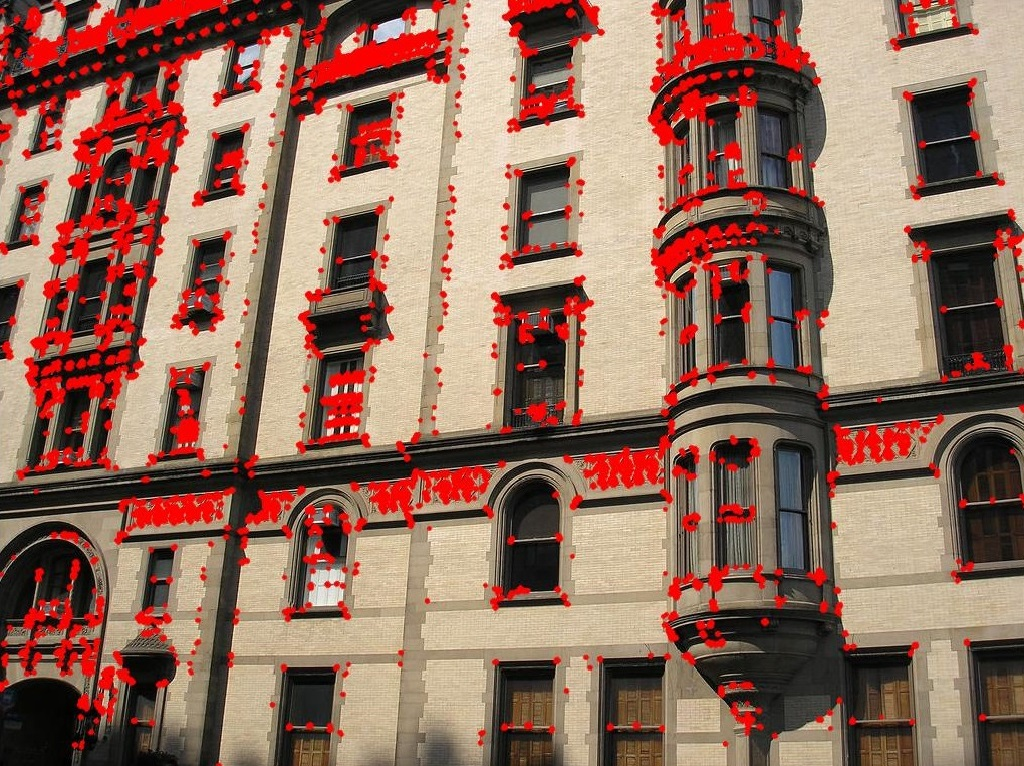
\includegraphics[width=0.33\textwidth]{1b1}
    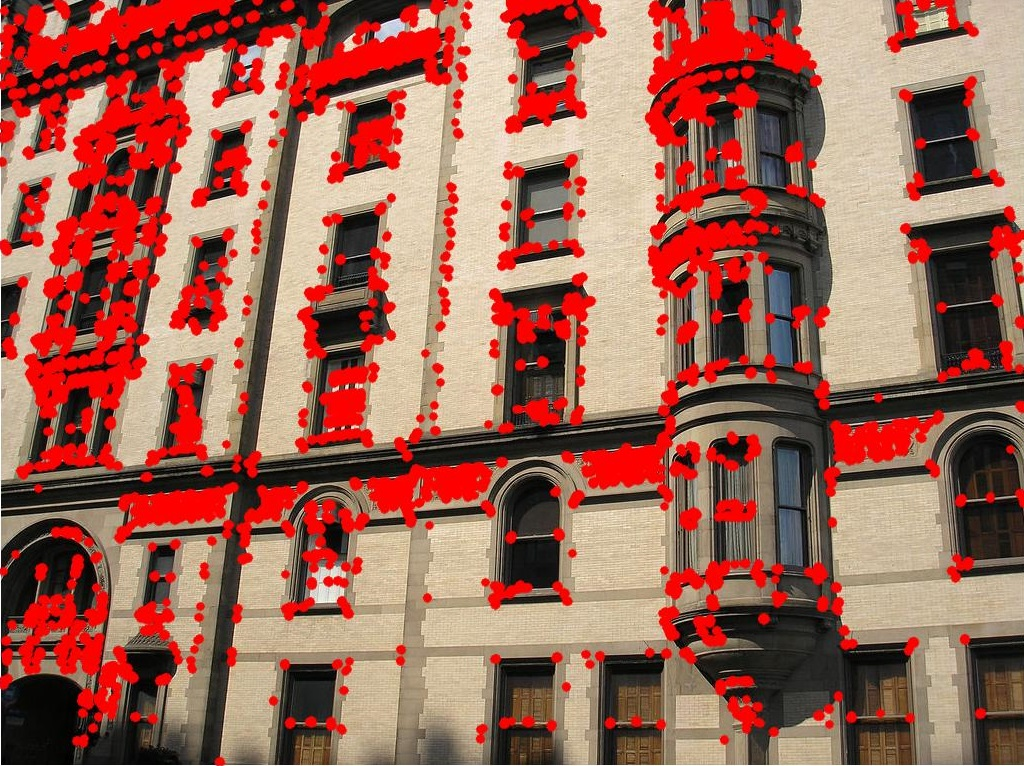
\includegraphics[width=0.33\textwidth]{1b3}
    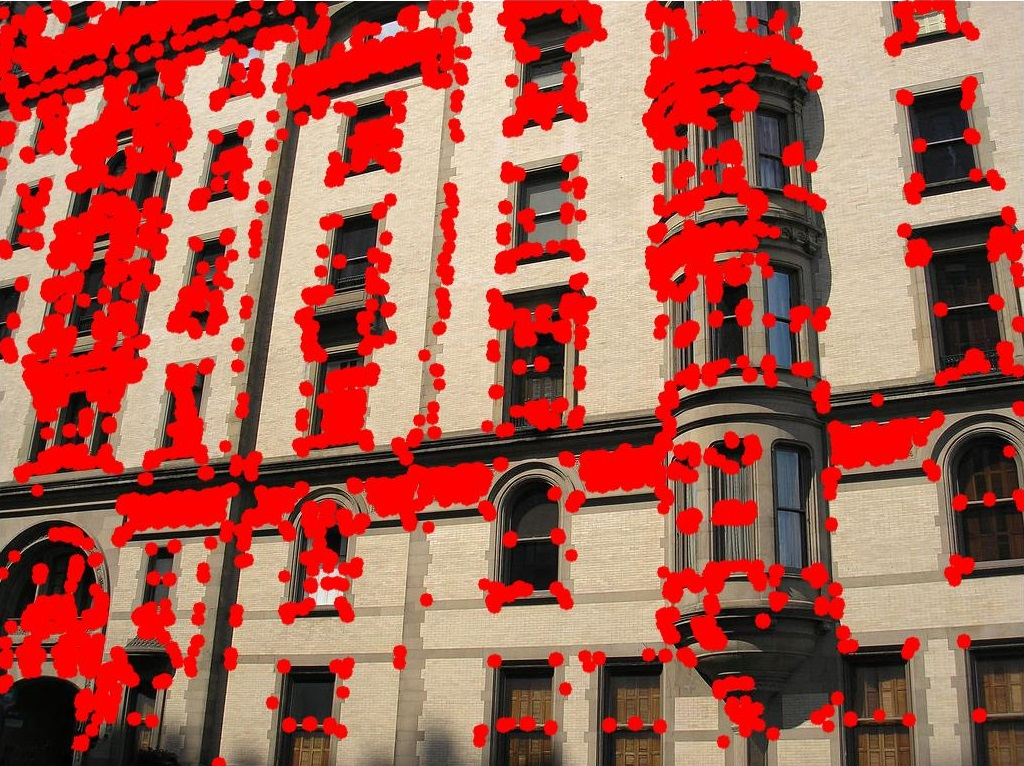
\includegraphics[width=0.33\textwidth]{1b5}
\end{figure}

\noindent
As the radius increase for the non maximum suppression filter, the size of the dot also gets bigger, because more neighboring values are being changed to its  local maximum by ordfilt2, as it reset the current value to the largest neighbor value, result in all neighbor values within the radius to exceed the threshold when actually just one pixel actually exceeds the threshold. \\
  
\newpage
\noindent
\textbf{1.c} \\
\begin{lstlisting}[
  mathescape,
  columns=fullflexible,
  basicstyle=\fontfamily{ttdefault}\selectfont,
]
im = imread('./synthetic.png');
img = rgb2gray(im);
imgS = img;%conv2(img,fspecial('Gaussian',[25 25],0.5),'same');%Base smoothing
k = 1.1;
sigma = 2.0;
s = k.^(1:10)*sigma;
responseLoG = zeros(size(img,1),size(img,2),length(s));

%% Filter over a set of scales %
for si = 1:length(s)
    sL = s(si);
    hs = max(25,min(floor(sL*3),300));
    HL = fspecial('log',[hs hs],sL);
    imgFiltL = conv2(double(imgS),double(HL),'same');
    %Compute the LoG
    responseLoG(:,:,si)  = (sL^2)*imgFiltL;
end

result = zeros(size(img));

[h,w,d] = size(responseLoG);
threshold = 20;

for x = 1:h
    for y = 1:w
        %Get the maxima over scale
        f = squeeze(responseLoG(x,y,:));
        %Maxima
        [fMax,fmaxLocs] = findpeaks(f);
        
        if (fMax > threshold)
           result(x,y) = 1;
        end
        
    end
    display(x);
end

[X, Y] = find(result == 1);
figure;
imshow(im);
hold on;
plot(Y ,X ,'R.');

\end{lstlisting}
\newpage
\begin{figure}[h]
  \caption{Result}
    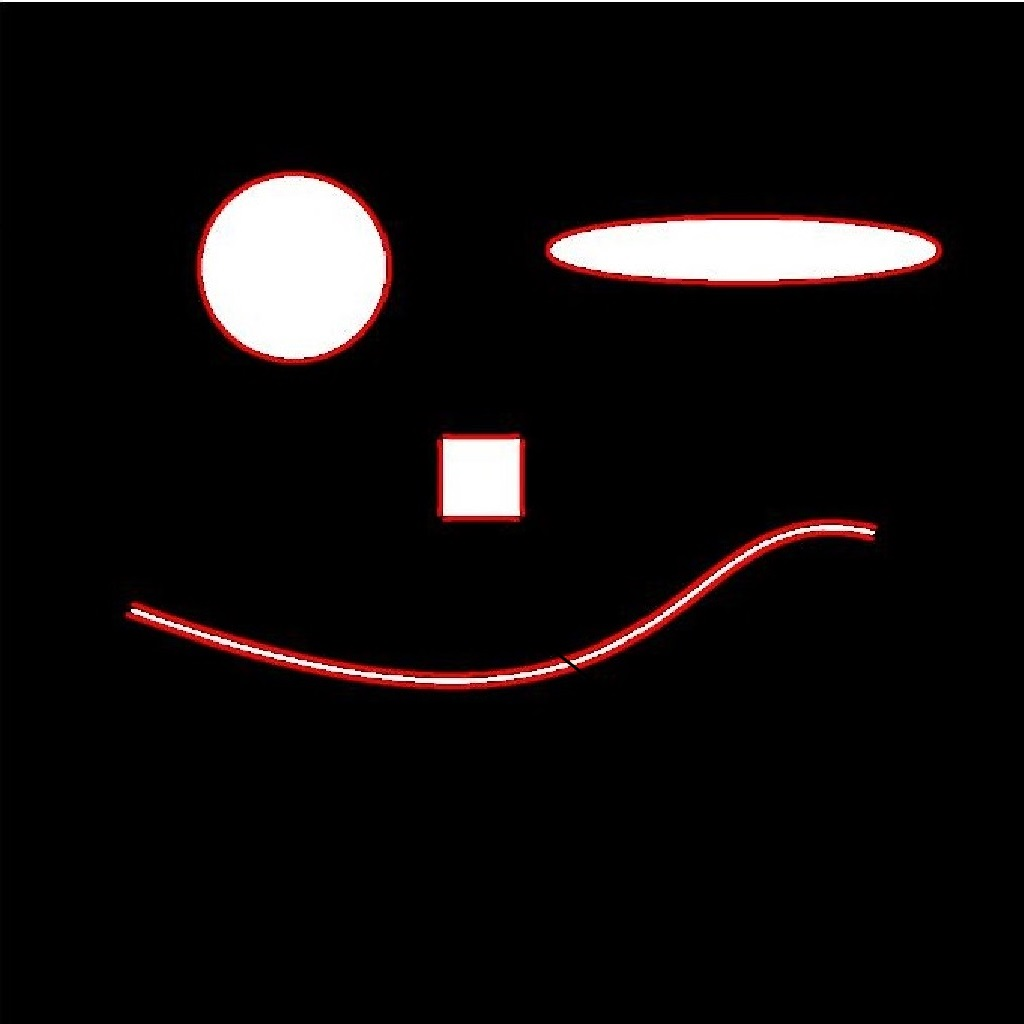
\includegraphics[width=1\textwidth]{1c}
\end{figure}

\newpage
\noindent
\textbf{1.d} \\

\begin{figure}[h]
  \caption{Harris Corner Metric}
    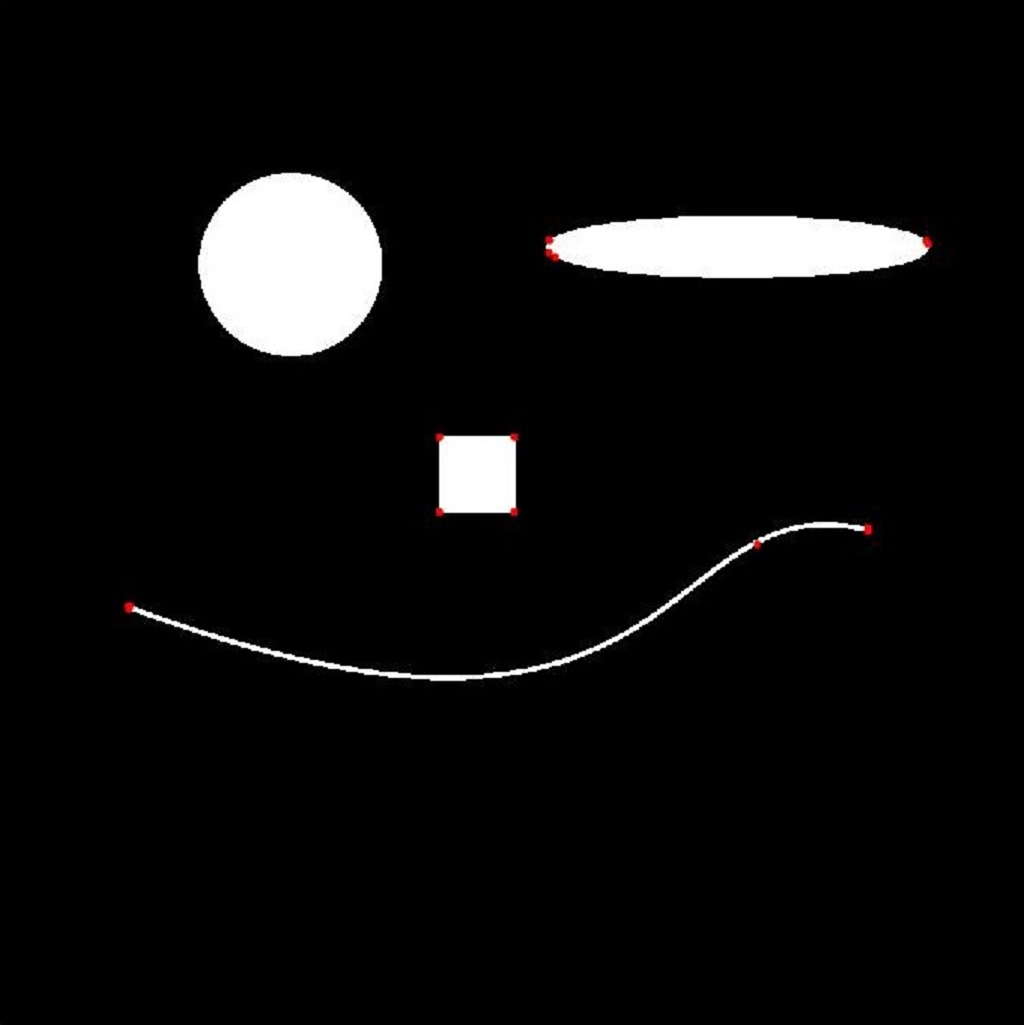
\includegraphics[width=0.45\textwidth]{1d3}
    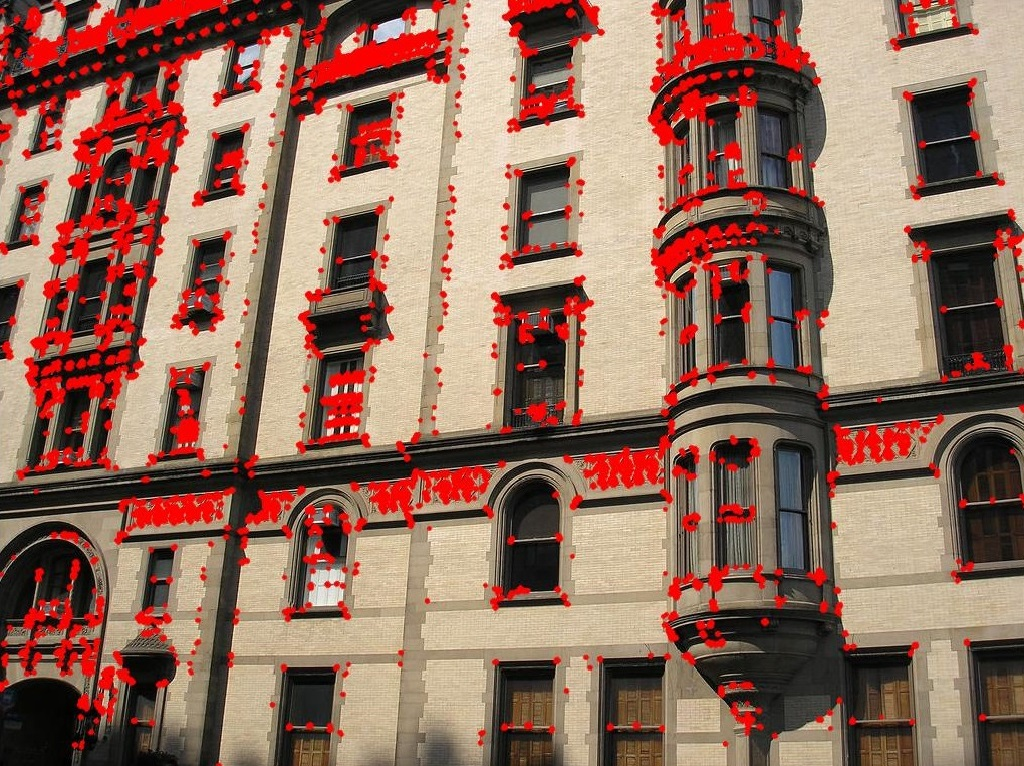
\includegraphics[width=0.55\textwidth]{1b1}
\end{figure}

\begin{figure}[h]
  \caption{Laplacian of Gaussian}
    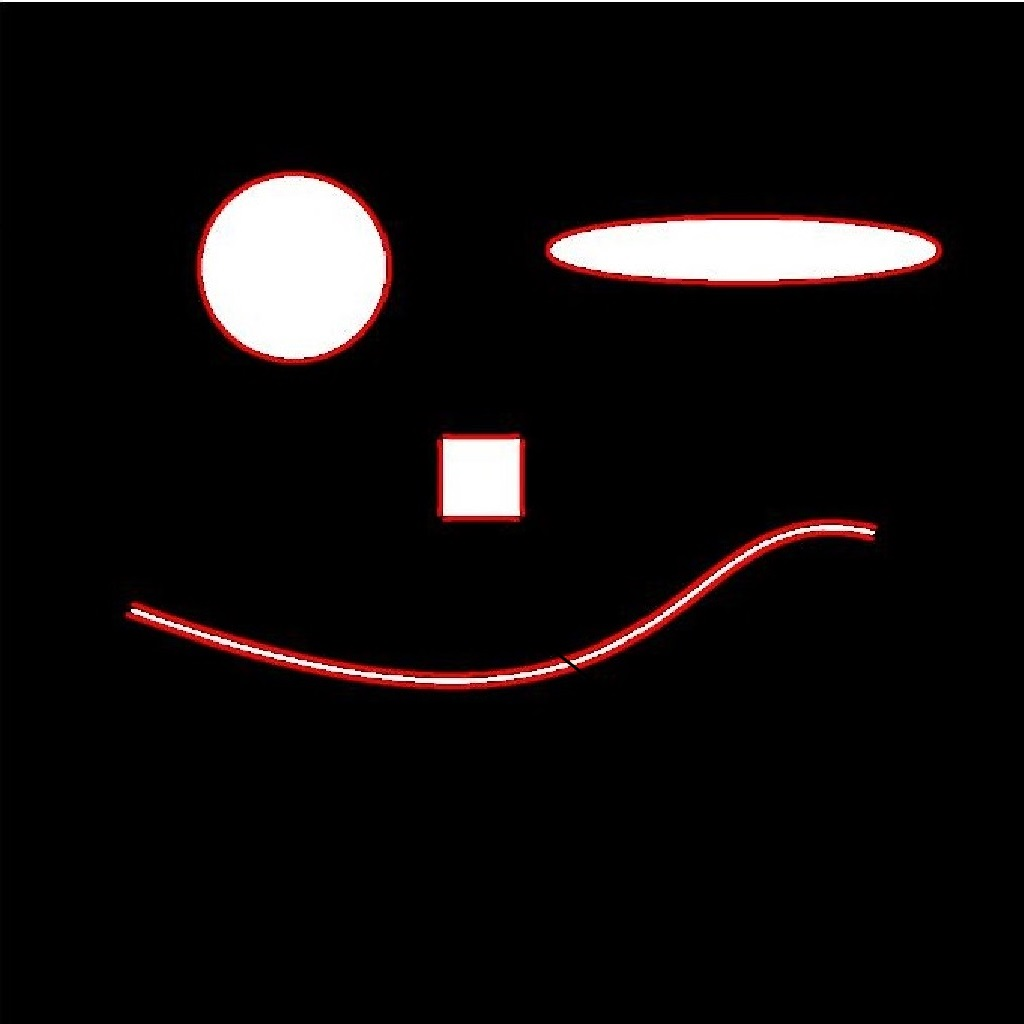
\includegraphics[width=0.45\textwidth]{1c}
    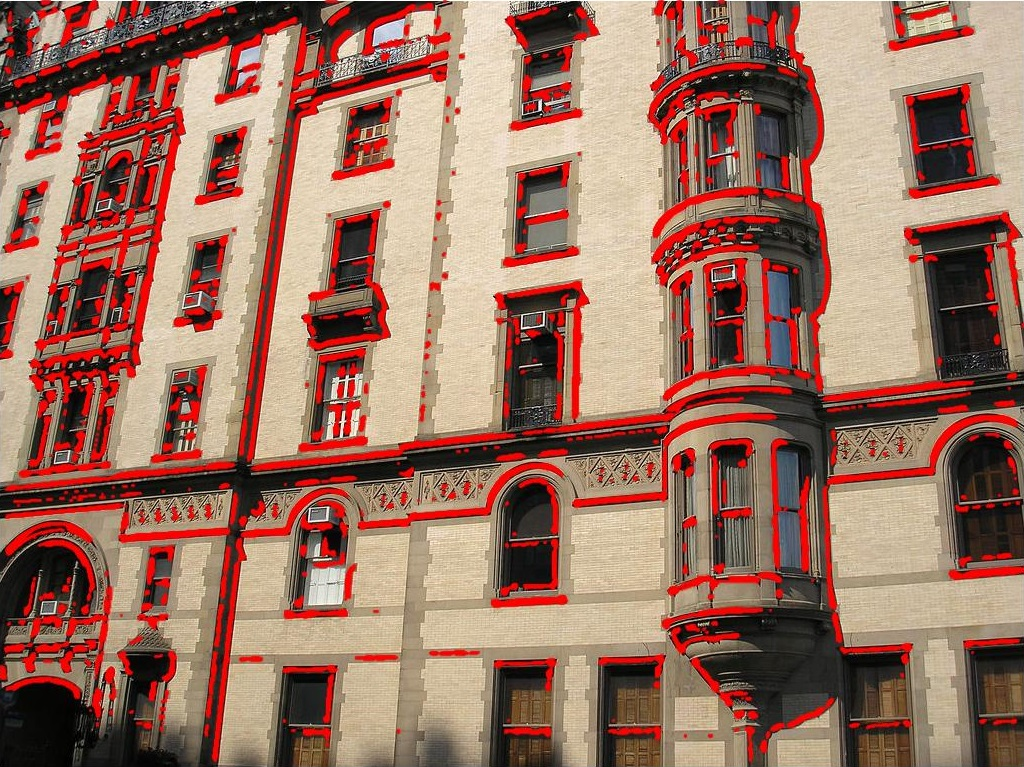
\includegraphics[width=0.55\textwidth]{1d2}
\end{figure}

\noindent
As from the 4 figures from above, we noticed that Harris Corner Metric didn't detect the left eye, because it is a circle, hence it couldn't find the corner.\\

\noindent
Same with the month, Harris Corner Metric only detected the side of the mouth but not the rest because it was smooth and the threshold wasn't low enough.\\

\noindent
On the other hand Laplacian of Gaussian method detect all of its eyes and nose, because there are blob, however, my algorithm isn't completely correct, and have detected many edges that are not necessarily corner. 

\newpage
\noindent
\textbf{2.a} \\
\begin{lstlisting}[
  mathescape,
  columns=fullflexible,
  basicstyle=\fontfamily{ttdefault}\selectfont,
]
book_img = imread('./book.jpg');
findbook_img = imread('./findBook.jpg');

book_img_gray = rgb2gray(book_img);
findbook_img_gray = rgb2gray(findbook_img);

run('F:/University/2016-2017/CSC420/Assignment/sift/toolbox/vl_setup');
[f1,d1] = vl_sift(im2single(book_img_gray));
p1 = subplot(1,2,1);
imshow(book_img);
h1 = vl_plotframe(f1);
h2 = vl_plotframe(f1);
set(h1,'color','k','linewidth',3);
set(h2,'color','y','linewidth',2);

[f2,d2] = vl_sift(im2single(findbook_img_gray));
p2 = subplot(1,2,2);
imshow(findbook_img);
h1 = vl_plotframe(f2);
h2 = vl_plotframe(f2);
set(h1,'color','k','linewidth',3);
set(h2,'color','y','linewidth',2);
\end{lstlisting}

\begin{figure}[h]
  \caption{Result}
    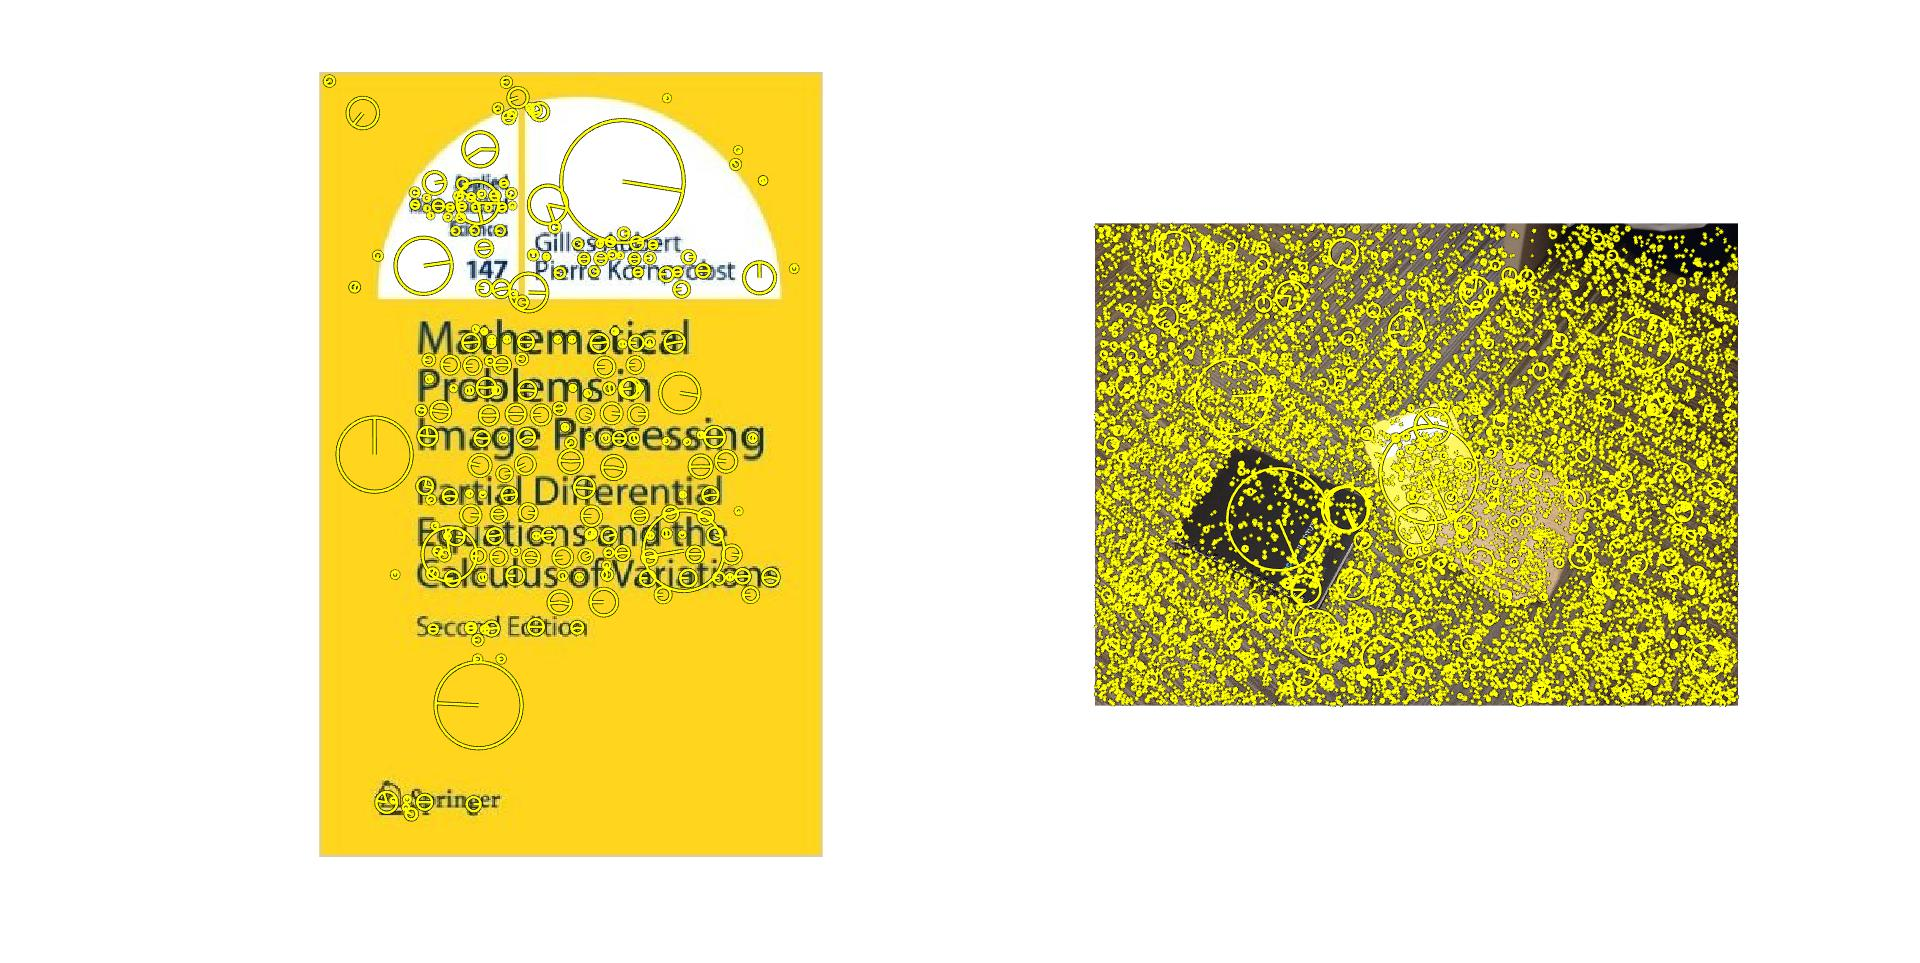
\includegraphics[width=1\textwidth]{2a}
\end{figure}

\end{document}
















